\documentclass[a4paper,12pt]{article}
\usepackage{xeCJK}          % 中文支持
\usepackage{fontspec}       % 英文/数学字体
\usepackage{amsmath, amssymb} % 数学公式
\usepackage{graphicx}       % 插入图片
\usepackage{hyperref}       % 目录超链接
\usepackage{geometry}       % 页面布局
\usepackage{bm}             % 粗体
\usepackage[table]{xcolor}  % 颜色
\usepackage{tabularx}       % 表格环境
\usepackage{tikz}           % TikZ 绘制主对角线斜线
\usepackage{tcolorbox}
\geometry{left=3cm,right=3cm,top=3cm,bottom=3cm}

% 抽离颜色和尺寸参数
\newcommand{\analysisTitleColor}{green!50!black}
\newcommand{\analysisBackColor}{white}
\newcommand{\analysisBoxRule}{0.8pt}
\newcommand{\analysisArc}{3pt}
\newcommand{\analysisPadding}{6pt}

% 定义 tcolorbox
\newtcolorbox{analysisbox}{
    title=解析,
    colback=\analysisBackColor,
    colframe=\analysisTitleColor,
    boxrule=\analysisBoxRule,
    arc=\analysisArc,
    left=\analysisPadding,
    right=\analysisPadding,
    top=4pt,
    bottom=4pt
}

% =========================
% 字体设置
% =========================
\setmainfont{Times New Roman}
\setsansfont{Helvetica Neue}
\setmonofont{Menlo}
\setCJKmainfont{PingFang SC}

% =========================
% 图形路径(可调整)
% =========================
\graphicspath{{./assets/}}

% =========================
% 文档开始
% =========================
\begin{document}

    \title{线性代数}
    \author{Bowen}
    \date{\today}
    \maketitle
    \tableofcontents
    \newpage

% =========================

    \section{行列式}

    \subsection{基础概念}
    \begin{enumerate}
        \item 由$1, 2, \dots, n$组成的有序数组程伟一个$n$阶排列,通常用$j_1, j_2, \dots, j_n$表示$n$阶排列
        \item 一个排列中,如果一个大的数排在小的数之前,就称这两个数构成\textbf{一个逆序},\textbf{一个排列的逆序总数称为这个排列的逆序数},用$\tau(j_1, j_2, \dots, j_n)$表示
        \item 如果一个排列的逆序数是偶数,则称这个排列为\textbf{偶排列},否则称为\textbf{奇排列}
    \end{enumerate}

    \subsection{性质}

    \begin{enumerate}
        \item 经转置行列式的值不变,即 $|A^T| = |A|$
        \item 某行元素全为 $0 \;\Rightarrow\;$ 行列式的值为 0
        \item 两行相等 $\Rightarrow$ 行列式的值为 0
        \item 两行成比例 $\Rightarrow$ 行列式的值为 0
        \item 某行(列)有公因数 $k$,可把 $k$ 提到行列式外
        \item 两行互换,行列式变号
        \item {\color{red}{\textbf{某行}}}所有元素都是两个数的和,则可写成两个行列式之和
        \item 某行的 $k$ 倍加至另一行,行列式的值不变
    \end{enumerate}

    \subsection{基础}

    \subsubsection{完全展开式}

    \begin{align*}
        \begin{vmatrix}
            a_{11} & a_{12} & \dots & a_{1n} \\
            a_{21} & a_{22} & \dots & a_{2n} \\
            \vdots & \vdots &       & \vdots \\
            a_{n1} & a_{n2} & \dots & a_{nn}
        \end{vmatrix}
        &= \sum_{j_1\,j_2\dots j_{n}} (-1)^{\tau(j_1\,j_2\dots j_n)} \mathbf{a_{1j_1}a_{2j_2}\dots a_{nj_n}} \\
        &= \sum_{\sigma \in S_n} (-1)^{\tau(\sigma)} \prod_{i=1}^{n} a_{i, \sigma(i)}
    \end{align*}

    \subsubsection{余子式 \& 代数余子式}

    \begin{enumerate}
        \item 在 $n$ 阶行列式中,划去元素 $a_{ij}$ 所在的第 $i$ 行、第 $j$ 列,由剩下的元素按原来的排法构成一个 $(n-1)$ 阶行列式,称为 $a_{ij}$ 的 \textbf{余子式},记为$\mathbf{M_{ij}}$;称$(-1)^{i+j}M_{ij}$为$a_{ij}$的\textbf{代数余子式},记为$\mathbf{A_{ij}}$,即
        \[
            A_{ij} = (-1)^{i+j}M_{ij}
        \]
        \item 三阶行列式的代数余子式
        \[
            A_{ij} =
            \begin{bmatrix}
                M_{11}  & -M_{12} & M_{13}  \\
                -M_{21} & M_{22}  & -M_{23} \\
                M_{31}  & -M_{32} & M_{33}
            \end{bmatrix}.
        \]
    \end{enumerate}

    \subsection{定理}

    \subsubsection{展开公式}

    \begin{enumerate}
        \item $n$阶行列式等于它的任意一行(列)的所有元素与他们各自对应的代数余子式的乘积之和,即
        \begin{align*}
            |A| &= a_{k1}A_{k1} + a_{k2}A_{k2} + \dots + a_{kn}A_{kn} (k=1,2,\dots,n)  & \text{行} \\
            &= a_{1k}A_{1k} + a_{2k}A_{2k} + \dots + a_{nk}A_{nk} (k=1,2,\dots,n)  & \text{列}
        \end{align*}
        \item 任意一行(列)的所有元素与其他行的代数余子式乘积之和为0,即
        \begin{align*}
            a_{i1}A_{k1} + a_{i2}A_{k2} + \dots + a_{in}A_{kn} = 0 &= 0  \quad  (i \neq k \text{且} i,k=1,2,\dots,n)   \\
            a_{1j}A_{1k} + a_{2j}A_{2k} + \dots + a_{nj}A_{nk} = 0 &= 0  \quad  (j \neq k \text{且} j,k=1,2,\dots,n)
        \end{align*}
    \end{enumerate}

    \subsubsection{乘法公式}
    设$\mathbf{A}$,$\mathbf{B}$都是$n$阶方阵,则
    \[
        |\mathbf{AB}| = |\mathbf{A}| \cdot |\mathbf{B}|
    \]

    \subsection{公式}

    \subsubsection{上(下)三角形}

    \begin{enumerate}
        \item 主对角线三角形
        \begin{align*}
            \begin{vmatrix}
                a_{11} & a_{12} & \dots  & a_{1n} \\
                & a_{22} & \dots  & a_{2n} \\
                &        & \ddots & \vdots \\
                &        &        & a_{nn}
            \end{vmatrix}
            = \begin{vmatrix}
                  a_{11} &        &        &        \\
                  a_{21} & a_{22} &        &        \\
                  \vdots & \vdots & \ddots &        \\
                  a_{n1} & a_{n2} & \dots  & a_{nn}
            \end{vmatrix}
            = a_{11}a_{22}\dots a_{nn}
        \end{align*}
        \item 副对角线三角形
        \begin{align*}
            \begin{vmatrix}
                a_{11} & a_{12} & \dots & a_{1,n-1} & a_{1n} \\
                a_{21} & a_{22} & \dots & a_{2,n-2} & 0      \\
                \vdots & \vdots &       & \vdots    & \vdots \\
                a_{n1} & 0      & \dots & 0         & 0
            \end{vmatrix}
            = \begin{vmatrix}
                  0      & \dots & 0         & a_{1n} \\
                  0      & \dots & a_{2,n-1} & a_{2n} \\
                  \vdots &       & \vdots    & \vdots \\
                  a_{n1} & \dots & a_{n,n-1} & a_{nn}
            \end{vmatrix}
            = (-1)^{\frac{n(n-1)}{2}}a_{1n}a_{2,n-2}\dots a_{n1}
        \end{align*}
    \end{enumerate}

    \subsubsection{拉普拉斯展开式}

    \begin{enumerate}
        \item 主对角线
        \[
            \renewcommand{\arraystretch}{1} % 缩小行距,避免竖线过高
            \setlength{\arraycolsep}{3pt}     % 调整列距
            \begin{vmatrix}
                \mathbf{A} & *          \\
                \mathbf{O} & \mathbf{B}
            \end{vmatrix}
            = \begin{vmatrix}
                  \mathbf{A} & \mathbf{O} \\
                  *          & \mathbf{B}
            \end{vmatrix}
            = |\mathbf{A}| \cdot |\mathbf{B}|
        \]
        \item 副对角线
        \[
            \renewcommand{\arraystretch}{1} % 缩小行距,避免竖线过高
            \setlength{\arraycolsep}{3pt}     % 调整列距
            \begin{vmatrix}
                *          & \mathbf{A} \\
                \mathbf{B} & \mathbf{O}
            \end{vmatrix}
            = \begin{vmatrix}
                  \mathbf{O} & \mathbf{A} \\
                  \mathbf{B} & *
            \end{vmatrix}
            = (-1)^{mn}|\mathbf{A}| \cdot |\mathbf{B}|
        \]
        \text{$m$,$n$分别是方阵$A$,$B$的阶数}
    \end{enumerate}

    \subsubsection{范德蒙行列式}

    \[
        \begin{vmatrix}
            1           & 1           & \dots & 1           \\
            x_1         & x_2         & \dots & x_n \\
            {x_1}^{2}   & {x_2}^2     & \dots & {x_n}^2     \\
            \vdots      & \vdots      &       & \vdots \\
            {x_1}^{n-1} & {x_2}^{n-1} & \dots & {x_n}^{n-1} \\
        \end{vmatrix}
        = \prod_{1 \le j < i \le n} (x_{i} - x_{j})
    \]

    \subsubsection{特征多项式}
    \begin{enumerate}
        \item 设$A = [a_{ij}]$是三阶矩阵,则$A$的特征多项式
        \[
            |A - \lambdaE| = -\lambda^3 + (a_{11} + a_{22} + a_{33})\lambda^2 - s_2 \lambda + |A|
        \]其中$s_2 =
        \begin{vmatrix}
            a_{11} & a_{12} \\
            a_{21} & a_{22}
        \end{vmatrix}
        +
        \begin{vmatrix}
            a_{11} & a_{13} \\
            a_{31} & a_{33}
        \end{vmatrix}
        +
        \begin{vmatrix}
            a_{22} & a_{23} \\
            a_{32} & a_{33}
        \end{vmatrix}.$
    \end{enumerate}

    \subsection{方阵行列式}

    \begin{enumerate}
        \item 若$A$是$n$阶矩阵,$A^T$是$A$的转置矩阵 \, \Rightarrow \, $|A^T| = |A|$
        \item 若$A$是$n$阶矩阵 \, \Rightarrow \, $|kA| = k^{n}|A|$
        \item 若$A$,$B$都是$n$阶矩阵 \, \Rightarrow \, $|AB| = |A||B|, |A^2| = |A|^2$
        \item 若$A$是$n$阶矩阵 \, \Rightarrow \, $|A^*| = |A|^{n-1}$
        \item 若$A$是$n$阶\textbf{可逆}矩阵 \, \Rightarrow \, $|A^{-1}| = |A|^{-1}$
        \item 若$A$是$n$阶矩阵,$\lambda_i(i = 1, 2, \cdots, n)$是$A$的特征值 \, \Rightarrow \, $|A| = \lambda_1 \lambda_2 \cdots \lambda_n$
        \item 若$n$阶矩阵$A$与$B$相似 \, \Rightarrow \, $|A| = |B|, |A + kE| = |B + kE|$
        \item
        \[
            \begin{vmatrix}
                A & B \\
                B & A
            \end{vmatrix}
            = \begin{vmatrix}
                  A + B & A + B \\
                  B     & A
            \end{vmatrix}
            = \begin{vmatrix}
                  A + B & 0     \\
                  B     & A - B
            \end{vmatrix}
            = |A + B| \cdot |A - B|
        \]
    \end{enumerate}

    \subsection{克拉默法则}

    设有 $n$ 元线性方程组:
    \[
        \begin{cases}
            a_{11}x_1 + a_{12}x_2 + \dots + a_{1n}x_n = b_1 \\
            a_{21}x_1 + a_{22}x_2 + \dots + a_{2n}x_n = b_2 \\
            \quad \vdots \\
            a_{n1}x_1 + a_{n2}x_2 + \dots + a_{nn}x_n = b_n
        \end{cases}
    \]

    记系数矩阵为 $\mathbf{A} = (a_{ij})_{n\times n}$,则其行列式为 $|\mathbf{A}|$。\textbf{若 $|\mathbf{A}| \neq 0$,则方程组有唯一解},并且第 $i$ 个未知数 $x_i$ 可由下式求得:

    \[
        x_i = \frac{|\mathbf{A}_i|}{|\mathbf{A}|}, \quad i=1,2,\dots,n
    \]

    其中 $\mathbf{A}_i$ 是将 $\mathbf{A}$ 的第 $i$ 列替换为常数列向量 $\mathbf{b} = (b_1, b_2, \dots, b_n)^T$ 后得到的矩阵,即:

    \[
        \mathbf{A}_i =
        \begin{pmatrix}
            a_{11} & \dots & b_1    & \dots & a_{1n} \\
            a_{21} & \dots & b_2    & \dots & a_{2n} \\
            \vdots &       & \vdots &       & \vdots \\
            a_{n1} & \dots & b_n    & \dots & a_{nn}
        \end{pmatrix}
    \]

    \paragraph{推论} 若齐次线性方程组:
    \[
        \begin{cases}
            a_{11}x_1 + a_{12}x_2 + \dots + a_{1n}x_n = 0 \\
            a_{21}x_1 + a_{22}x_2 + \dots + a_{2n}x_n = 0 \\
            \quad \vdots \\
            a_{n1}x_1 + a_{n2}x_2 + \dots + a_{nn}x_n = 0
        \end{cases}
    \]

    \begin{enumerate}
        \item 系数行列式$|A| \neq 0$ $\Leftrightarrow$ 方程组\textbf{只有零解}
        \item 系数行列式$|A| = 0$ $\Leftrightarrow$ 方程组\textbf{有非零解}
    \end{enumerate}

    \subsection{方法步骤}

    \begin{enumerate}
        \item 对于\textbf{主对角线爪型}行列式,可用\textbf{主}对角线元素将其化为上(下)三角型来计算
        \[
            \begin{bmatrix}
                1 & 1 & 1 & 1 \\
                1 & 2 & 0 & 0 \\
                1 & 0 & 3 & 0 \\
                1 & 0 & 0 & 4
            \end{bmatrix}
        \]
        \item 对于\textbf{副对角线爪型}行列式,可用\textbf{副}对角线元素将其化为\textbf{反上(下)三角型}来计算
        \[
            \begin{bmatrix}
                1 & 1 & 1 & 1 \\
                0 & 0 & 2 & 1 \\
                0 & 3 & 0 & 1 \\
                4 & 0 & 0 & 1
            \end{bmatrix}
        \]
        \item 把各行(列)均加到第一行(列)
        \item 逐行(列)相加
        \item 若有较多$0$,可考虑直接用行(列)展开公式
        \item 特殊的\textbf{三对角线}行列式
        \begin{enumerate}
            \item 三角化法: 逐行相加,构造上下三角型
            \item 递推法
            \item 归纳法
        \end{enumerate}
        \item 数学归纳法
        \begin{itemize}
            \item \textbf{普通数学归纳法(Mathematical Induction)}
            \begin{enumerate}
                \item 验证 $n = 1$ 时,命题 $f_n$ 成立;
                \item 假设 $n = k$ 时,命题 $f_n$ 成立;
                \item 证明 $n = k + 1$ 时,命题 $f_n$ 成立。
            \end{enumerate}

            \item \textbf{强(完全)归纳法(Strong Induction)}
            \begin{enumerate}
                \item 验证 $n = 1$ 和 $n = 2$ 时,命题 $f_n$ 成立;
                \item 假设当 $n < k$ 时,命题 $f_n$ 均成立;
                \item 证明 $n = k$ 时,命题 $f_n$ 成立。
            \end{enumerate}
        \end{itemize}
    \end{enumerate}

    \subsection{条件转换思路}

    \begin{enumerate}
        \item 齐次方程组$Ax = 0$有非零解
        \begin{align*}
            &\Leftrightarrow\; r(A) < n (\text{其中}n = \text{未知数的个数})  \\
            &\Leftrightarrow\; |A| = 0  \\
            &\Leftrightarrow\; A \text{的列向量组线性相关}  \\
        \end{align*}
    \end{enumerate}

    \subsection{理解}

    \begin{enumerate}
    \end{enumerate}

    \section{矩阵}

    \subsection{基础概念}

    \begin{enumerate}
        \item $m$行$n$列表格称为$m \times n$矩阵,当 $m = n$ 时,矩阵$A$称为$n$阶矩阵或\textbf{$n$阶方阵}
        \item 如果一个矩阵的所有元素都是$0$,则称这个矩阵是\textbf{零矩阵},可简记为$\mathbf{O}$
        \item 如果一个方阵,所有非主对角线元素都是0,则称这个矩阵是\textbf{对角矩阵}
        \item 两个$m \times n$型矩阵$A = [a_{ij}]$,$B = [b_{ij}]$,如果对应的元素都相等,即$a_{ij} = b_{ij}(i = 1,2,\dots,m; j = 1,2,\dots,n)$,则称矩阵$A$与$B$相等,记作$A = B$
        \item $n$阶方阵$A = [a_{ij}]_{n \times n}$的元素所构成的行列式称为$n$阶方阵$A$的行列式,记作$|A|$或$\det A$
        \item 把矩阵$A$的行换成同序数的列得到一个新矩阵,称为矩阵$A$的\textbf{转置矩阵},记作$A^T$
        \item 如果方阵$A$满足$A^T = A$,则称$A$是\textbf{对称矩阵},即$a_{ij} = a_{ji}$
        \item 如果方阵$A$满足$A^T = -A$,则称$A$是\textbf{反对称矩阵},即$a_{ij} = -a_{ji}$
        \item $n$阶方阵$A = [a_{ij}]_{n \times n}$,行列式$|A|$的每个元素$a_{ij}$的代数余子式$A_{ij}$所构成的如下矩阵
        \[
            A^* =
            \begin{bmatrix}
                A_{\color{red}{11}} & A_{\textcolor[rgb]{0.2, 0.6, 0.3}{21}} & \dots & A_{\textcolor{blue}{n1}} \\
                A_{\color{red}{12}} & A_{\textcolor[rgb]{0.2, 0.6, 0.3}{22}} & \dots & A_{\textcolor{blue}{n2}} \\
                \vdots              & \vdots                                 &       & \vdots                   \\
                A_{\color{red}{1n}} & A_{\textcolor[rgb]{0.2, 0.6, 0.3}{2n}} & \dots & A_{\textcolor{blue}{nn}}
            \end{bmatrix}
        \]
        称为矩阵$A$的\textbf{伴随矩阵}
        \item 伴随矩阵是余子式矩阵的转置,即$A^* = [A_{ji}] = (A_{ij})^T$
        \item $n$阶方阵$A = [a_{ij}]_{n \times n}$,如果存在$n$阶方阵$B$使得$AB = BA = E$(单位矩阵)成立,则称$A$是\textbf{可逆矩阵}或\textbf{非奇异矩阵},$B$是$A$的逆矩阵
        \item 对$m \times n$矩阵,下列三种变换
        \begin{enumerate}
            \item 用非零常数$k$乘矩阵的某一行(列)
            \item 互换矩阵某两行(列)的位置
            \item 把某行(列)的$k$倍加至另一行(列)
        \end{enumerate}
        称为矩阵的\textbf{初等行(列)变换},统称为矩阵的\textbf{初等变换}
        \item 如果矩阵$A$经过有限次初等变换变成矩阵$B$,则称矩阵$A$与矩阵$B$\textbf{等价},记作$A \overset{\sim}{=} B$
        \item 单位矩阵经过一次初等变换等到的矩阵称为\textbf{初等矩阵}
        \begin{enumerate}
            \item $E_{i}(k)$ 单位矩阵第$i$行乘以常数$k$
            \item $E_{ij}$ 单位矩阵互换$i,j$行
            \item $E_{ij}(k)$ 单位矩阵第$j$行的$k$倍加至第$i$行
        \end{enumerate}
        \item 设$\alpha = (a_1, a_2, \dots, a_n)^{T}$,$\beta = (b_1, b_2, \dots, b_n)^{T}$。向量内积为
        \[
            (\alpha, \beta) = \alpha^{T}\beta = \beta^{T}\alpha = a_{1}b_{1} + a_{2}b_{2} + \dots + a_{n}b_{n}
        \]
        \item 向量$\alpha = (a_1, a_2, \dots, a_n)^{T}$的长度
        \[
            ||\alpha|| = \sqrt{\alpha^T\alpha} = \sqrt {a_1^2 + a_2^2 + \dots + a_n^2}
        \]
        \item 若$(\alpha, \beta) = 0$即$a_{1}b_{1} + a_{2}b_{2} + \dots + a_{n}b_{n} = 0$,则称$\alpha$与$\beta$正交,记为$\alpha \perp \beta$
        \item 设 $A$ 是 $n$ 阶矩阵,满足 $AA^{T} = A^{T}A = E$,称 $A$ 是 \textbf{正交矩阵:}
        \begin{align*}
            &\Leftrightarrow\; A^{T} = A^{-1} \\
            &\Leftrightarrow\; A \text{ 的行(列)向量两两正交(单位向量)} \\
            &\Leftrightarrow\; A \text{ 的每个行(列)向量长度均为1} \\
            &\Leftrightarrow\; A \text{ 的行(列)向量平方和为 1} \\
            &\Leftrightarrow\; a_{1}^2 + a_{2}^2 + \dots + a_{n}^2 = 1 \\
            &{\color{red}{\Rightarrow}}\; |A|^{2} = 1 \;\;\Leftrightarrow\;\; |A| = 1 \text{ 或 } |A| = -1
        \end{align*}
        \item 若 $A$ 是正交矩阵且 $A = (\alpha_1,\alpha_2,\dots,\alpha_n)$,则:
        \begin{enumerate}
            \item $\alpha_{i}^{T}\alpha_{i} = 1$
            \item $\alpha_{i}^{T}\alpha_{j} = 0 \; (i \neq j)$
        \end{enumerate}
        \item 在$m \times n$矩阵$A$中,任取$k$行与$k$列$(k \le m, k \le n)$,位于这个行与列的交叉点上的$k^2$个元素按其在原来矩阵$A$中的次序可构成一个$k$阶行列式,称其为矩阵$A$的一个$k$阶\textbf{子式}
        \item 矩阵$A$的非零子式的最高阶数称为矩阵$A$的{\color[rgb]{0.2, 0.6, 0.3}{秩}},记为$r(A)$。零矩阵的秩规定为$0$
        \item 矩阵秩的理解
        \begin{enumerate}
            \item $r(A) = r$ \Leftrightarrow A \text{中\textcolor[rgb]{0.2, 0.6, 0.3}{有}}r\text{阶子式不为}0\text{,\textcolor[rgb]{0.2, 0.6, 0.3}{任何}}r + 1\text{阶子式(若存在)必\textcolor[rgb]{0.2, 0.6, 0.3}{全}为}0
            \item $r(A) < r$ \Leftrightarrow A \text{中\textcolor[rgb]{0.2, 0.6, 0.3}{每}一个}r\text{阶子式\textcolor[rgb]{0.2, 0.6, 0.3}{全}为}0
            \item $r(A) \ge r$ \Leftrightarrow A \text{中\textcolor[rgb]{0.2, 0.6, 0.3}{有}}r\text{阶子式不为}0
            \item $r(A) = 0$ \Leftrightarrow A = \mathbf{O}
            \item $r(A) \neq \mathbf{O}$ \Leftrightarrow 1 \le r(A) \le n
            \item 若$A$是$n$阶矩阵
            \begin{itemize}
                \item $r(A) = n$ \Leftrightarrow |A| \neq 0 \Leftrightarrow A\text{可逆}
                \item $r(A) < n$ \Leftrightarrow |A| = 0 \Leftrightarrow A\text{不可逆}
            \end{itemize}
            \item 若$A$是$m \times n$阶矩阵 \Leftrightarrow r(A) \le min(m, n)
        \end{enumerate}
    \end{enumerate}

    \subsection{定理}

    \begin{enumerate}
        \item 若$A$是可逆矩阵,则矩阵$A$的逆矩阵\textbf{唯一},记为$A^{-1}$
        \item $n$ 阶矩阵$A$可逆
        \begin{align*}
            &\Leftrightarrow\; |A| \neq 0  \\
            &\Leftrightarrow\; r(A) = n  \\
            &\Leftrightarrow\; A \text{的列(行)向量组线性无关}  \\
            &\Leftrightarrow\; A = P_{1}P_{2}\dots P_{s}, P_{i}(i = 1,2,\dots,s)\text{是初等矩阵}  \\
            &\Leftrightarrow\; A \text{通过初等变换能化为单位矩阵}  \\
            &\Leftrightarrow\; A \text{与单位矩阵等价}  \\
            &\Leftrightarrow\; 0\text{不是矩阵} A \text{的特征值}  \\
            &\Leftrightarrow\; \text{齐次线性方程组} Ax = 0 \text{只有零解}  \\
        \end{align*}
        \item $n$ 阶矩阵$A${\color{red}{不可逆}}
        \begin{align*}
            &\Leftrightarrow\; |A| = 0  \\
            &\Leftrightarrow\; r(A) < n  \\
            &\Leftrightarrow\; A \text{的列(行)向量组线性相关}  \\
            &\;\Leftrightarrow\; A \text{无法表示为初等矩阵的乘积} \\
            &\Leftrightarrow\; A \text{无法通过初等变换能化为单位矩阵}  \\
            &\Leftrightarrow\; 0\text{是矩阵} A \text{的特征值}  \\
            &\Leftrightarrow\; \text{齐次线性方程组} Ax = 0 \text{有非零解}
        \end{align*}
        \item $A \overset{\sim}{=} B$
        \begin{align*}
            &\Leftrightarrow\; r(A) = r(B)  \\
            &\Leftrightarrow\; A \text{通过初等变换能化为} B  \\
            &\Rightarrow\; |A| = 0 \Leftrightarrow |B| = 0, |A| \neq 0 \Leftrightarrow |B| \neq 0. \text{即}A\;B\text{的行列式同时为0或同时不为0}  \\
        \end{align*}
        \item 若$A$是$n$阶矩阵,且满足$AB = E$,则必有$BA = E$
        \item 用初等矩阵$P$左(右)乘矩阵$A$,其结果$PA$($AP$)就是对矩阵$A$作一次相应的初等行(列)变换 \; \Rightarrow \textbf{左乘行变换,右乘列变换}
        \item 初等矩阵均可逆,其逆矩阵是同类型的初等矩阵,即

        \renewcommand{\arraystretch}{1.2}  % 行高放大 1.2 倍
        \begin{tabularx}{\textwidth}{l c >{\raggedright\arraybackslash}X}
            倍乘 & $E_i^{-1}(k) = E_i(1/k)$      & 第 $i$ 行(或列)乘以非零常数 $k$ 的逆矩阵是第 $i$ 行(或列)乘以 $1/k$                     \\
            互换 & $E_{ij}^{-1} = E_{ij}$        & 交换第 $i$ 行(或列)和第 $j$ 行(或列)的\textbf{\color{red}{逆矩阵是其本身}}            \\
            倍加 & $E_{ij}^{-1}(k) = E_{ij}(-k)$ & 第 $i$ 行(或列)加上 $k$ 倍第 $j$ 行(或列)的逆矩阵是第 $i$ 行(或列)加上 $-k$ 倍第 $j$ 行(或列) \\
        \end{tabularx}
        \item 矩阵$A$与$B$\textbf{等价}的充分必要条件是存在可逆矩阵$P$与$Q$,使$PAQ = B$
        \item 秩$r(A) = A \text{的列秩} = A \text{的行秩}$
        \item 矩阵经初等变换后秩不变
    \end{enumerate}

    \subsection{运算}

    \begin{enumerate}
        \item 设$A = [a_{ij}]$,$B = [b_{ij}]$是两个$m \times n$矩阵,则$m \times n$矩阵$C = [c_{ij}] = [a_{ij} + b_{ij}]$称为矩阵$A$与$B$的和,记作$A + B = C$
        \item 设$A = [a_{ij}]$是$m \times n$矩阵,$k$是一个常数,则$m \times n$矩阵$[ka_{ij}]$称为数$k$与矩阵$A$的\textbf{数乘},记作$kA$
        \item 设$A, B, C, \mathbf{O}$都是$m \times n$矩阵,$k, l$是常数,则矩阵的加法和数乘运算满足:
        \begin{enumerate}
            \item $A + B = B + A$
            \item $(A + B) + C = A + (B + C)$
            \item $A + \mathbf{O} = A$
            \item $A + (-A) = \mathbf{O}$
            \item $1A = A$
            \item $k(lA) = (kl)A$
            \item $(kA)^n = k^{n}A^n$
            \item $k(A + B) = kA + kB$
            \item $(k + l)A = kA + lA$
        \end{enumerate}
        \item 设$A = [a_{ij}]$是$m \times n$矩阵,$B = [b_{ij}]$是$n \times s$矩阵,那么$m \times s$矩阵$C = [c_{ij}]$,其中
        \[
            c_{ij} = a_{i1}b_{1j} + a_{i2}b_{2j} + \dots + a_{in}b_{nj} = \sum_{k=1}^{n} a_{ik}b_{kj} = \sum \text{第$i$行} \times \text{第$j$列}
        \]
        称为$A$与$B$的\textbf{乘积},记作$C = AB$
        \item 矩阵乘法有下列法则:
        \begin{enumerate}
            \item $A(BC) = (AB)C$
            \item $A(B + C) = AB + AC$
            \item $(A + B)C = AC + BC$
            \item $(kA)(lB) = klAB$
            \item $AE = EA = A$
            \item $\mathbf{O}A = A\mathbf{O} = \mathbf{O}$
        \end{enumerate}
        \item 设$A$是$n$阶矩阵,$k$是正整数,
        \begin{enumerate}
            \item $A$的$k$次方幂$A^k = A \cdot A \dots A$($k$个$A$)
            \item $\mathbf{A^0 = E}$
            \item $A^k \cdot A^l = A^{k+l}$
            \item $(A^k)^l = A^{kl}$
        \end{enumerate}
        \item
        \[
            \begin{bmatrix}
                A_1 & A_2 \\
                A_3 & A_4
            \end{bmatrix}
            + \begin{bmatrix}
                  B_1 & B_2 \\
                  B_3 & B_4
            \end{bmatrix}
            = \begin{bmatrix}
                  A_1 + B_1 & A_2 + B_2 \\
                  A_3 + B_3 & A_4 + B_4
            \end{bmatrix}
        \]
        \item
        \[
            \begin{bmatrix}
                A & B \\
                C & D
            \end{bmatrix}
            \begin{bmatrix}
                X & Y \\
                Z & W
            \end{bmatrix}
            = \begin{bmatrix}
                  AX + BZ & AY + BW \\
                  CX + DZ & CY + DW
            \end{bmatrix}
        \]
        \item
        \[
            \begin{bmatrix}
                A & B \\
                C & D
            \end{bmatrix}^{T}
            = \begin{bmatrix}
                  A^T & C^T \\
                  B^T & D^T
            \end{bmatrix}
        \]
        \item $(A + B)^2 = (A + B)(A + B) = A^2 + {\color{red}{AB}} + {\color{red}{BA}} + B^2 \;\mathbf{\neq}\; A^2 + 2AB + B^2$
        \item $\color[rgb]{0.2, 0.6, 0.3}{\mathbf{(A + E)^2 = A^2 + 2A + E}}$
        \begin{enumerate}
            \item $E - A^3 = (E - A)(E + A + A^2)$
            \item $E + A^3 = (E + A)(E - A + A^2)$
            \item $AB - 2B - 4A = 0$ \Leftrightarrow \; $(A - 2E)(B - 4E) = 8E$
        \end{enumerate}
        \item 设$\alpha$和$\beta$都是列向量,则
        \begin{enumerate}
            \item 列向量 \cdot \text{行向量:} \, $\alpha\beta^T = (\beta\alpha^T)^T$,两者都是$n$阶矩阵(互为转置)
            \item 行向量 \cdot \text{列向量:} \, $\alpha^T\beta = \beta^T\alpha$ 是一个\textbf{数}
            \item
            \[
                \alpha\alpha^T =
                \begin{bmatrix}
                    a_1^2   & a_1 a_2 & a_1 a_3 & \dots  & a_1 a_n \\
                    a_1 a_2 & a_2^2   & a_2 a_3 & \dots  & a_2 a_n \\
                    a_1 a_3 & a_2 a_3 & a_3^2   & \dots  & a_3 a_n \\
                    \vdots  & \vdots  & \vdots  & \ddots & \vdots  \\
                    a_1 a_n & a_2 a_n & a_3 a_n & \dots  & a_n^2
                \end{bmatrix} \textbf{(对称矩阵)}
            \]
            \item $\color{red}{r(\alpha\alpha^T) = 1}$
            \item $\alpha\alpha^T$特征值是{\color{red}{$||\alpha||^2, 0, 0, \dots, 0(n - 1\text{个})$}}
            \item
            \[
                \alpha^T \alpha = a_1^2 + a_2^2 + \dots + a_n^2 = \sum_{k=1}^{n} a_k^2 \quad \text{(平方和)}
            \]
        \end{enumerate}
        \item 向量
        \begin{itemize}
            \item $(\alpha, \beta) = (\beta, \alpha)$
            \item $(k\alpha, \beta) = (\alpha, k\beta) = k(\alpha, \beta)$
            \item $(\alpha + \beta, \gamma) = (\alpha, \gamma) + (\beta, \gamma)$
            \item $(\alpha, \beta + \gamma) = (\alpha, \beta) + (\alpha, \gamma)$
            \item $(\alpha, \alpha) \ge 0$
        \end{itemize}
    \end{enumerate}

    \subsection{公式}

    \subsubsection{行列式}

    \begin{enumerate}
        \item $|A^T| = |A|$
        \item $|kA| = k^{n}|A|$
        \item $|AB| = |A||B|$ \;\text{,} $|A^2| = |A|^2$
        \item \color{red}{$|A^*| = |A|^{n-1}$}
        \item $|A^{-1}| = |A|^{-1}$
    \end{enumerate}

    \subsubsection{转置}

    \begin{enumerate}
        \item $(A^T)^T = A$
        \item $(A + B)^T = A^T + B^T$
        \item $(A - B)^T = A^T - B^T$
        \item $(kA)^T = kA^T$
        \item $(AB)^T = B^{T}A^T $
        \item $(E + A)^T = E + A^T $
    \end{enumerate}

    \subsubsection{伴随}

    \begin{enumerate}
        \item $(A^*)^{-1} = (A^{-1})^* = \frac{1}{|A|}A$
        \item $AA^{*} = A^{*}A = |A|E$
        \item $A^{*} = |A|A^{-1}$
        \item $A$可逆有$|A^*| = |A|^{n-1}$
        \item $(AB)^* = B^{*}A^*$
        \item $(A^*)^T = (A^T)^*$
        \item $(kA)^* = k^{n-1}A^*$
        \item $(A^*)^* = |A|^{n-2}A$
        \begin{enumerate}
            \item 若$A$不可逆($|A| = 0$),则
            \begin{enumerate}
                \item 且$n \ge 3$时,$(A^*)^* = O$
                \item 且$n = 2$时,$(A^*)^* = A$
            \end{enumerate}
        \end{enumerate}
        \item
        \begin{flalign*}
            r(A^*) &=
            \begin{cases}
                n, & \text{如果 } r(A) = n, \\
                1, & \text{如果 } r(A) = n - 1, \\
                0, & \text{如果 } r(A) < n - 1
            \end{cases} &&
        \end{flalign*}
        \item 设$A = \begin{bmatrix}
                         a & b \\
                         c & d
        \end{bmatrix}$(二阶矩阵),则$A^* = \begin{bmatrix}
                                              d  & -b \\
                                              -c & a
        \end{bmatrix}$。\textbf{主对调,副变号}
    \end{enumerate}

    \subsubsection{可逆}

    \begin{enumerate}
        \item $(A^{-1})^{-1} = A$
        \item $(kA)^{-1} = \frac{1}{k}A^{-1}(k \neq 0)$
        \item $(AB)^{-1} = B^{-1}A^{-1}$
        \item $(ABC)^{-1} = C^{-1}B^{-1}A^{-1}$
        \item $(A^n)^{-1} = (A^{-1})^n$
        \item $(A^{-1})^T = (A^T)^{-1}$
        \item $A^{-1} = \frac{1}{|A|}A^{*}$
        \item $|A^{-1}| = \frac{1}{|A|} \Rightarrow |P^{-1}||P| = 1$
        \item
        \[
            \begin{bmatrix}
                a & b \\
                c & d
            \end{bmatrix}^{-1}
            = \frac{1}{ad - bc}\begin{bmatrix}
                                   d  & -b \\
                                   -c & a
            \end{bmatrix}
        \]
        \item
        \[
            \begin{bmatrix}
                &   & a \\
                & b &   \\
                c &   &   \\
            \end{bmatrix}^{-1}
            = \begin{bmatrix}
                  &             & \frac{1}{c} \\
                  & \frac{1}{b} &             \\
                  \frac{1}{a} &             &             \\
            \end{bmatrix}
        \]
    \end{enumerate}

    \subsubsection{秩}

    \begin{enumerate}
        \item $r(A) = r(A^T) = r(A^{T}A) = r(AA^{T})$
        \item 当$k \neq 0$时,$r(kA) = r(A)$
        \item $r(A + B) \le r(A, B) \le r(A) + r(B)$
        \item $A$是$m \times n$矩阵,$B$是$n \times s$矩阵,则
        \begin{enumerate}
            \item $r(AB) \le r(A) \text{并且} r(AB) \le r(B)$,即 $r(AB) \le \min(r(A), r(B))$
            \item $r(A) + r(B) - n \le r(AB)$
            \item $\color{red}{r(A, AB) = r(A)}$详见理解1
            \item $\color{red}{r(B, BA) = r(B)}$
            \item 且$AB = O$,则
            \begin{enumerate}
                \item $r(A) + r(B) {\color{red}{\le}} n$
                \item $B$ 的列向量是齐次方程组 $Ax = 0$ 的解
                \begin{itemize}
                    \item 按列分块,有
                    \[
                        B = [b_1, b_2, \dots, b_s], \\
                        AB = A[b_1, b_2, \dots, b_s] = [Ab_1, Ab_2, \dots, Ab_s] = [0, 0, \dots, 0]
                    \]
                    因此
                    \[
                        Ab_i = 0, \quad i = 1, 2, \dots, s.
                    \]
                \end{itemize}
            \end{enumerate}
            \item 且$AB = C$,则
            \begin{enumerate}
                \item {\color[rgb]{0.2, 0.6, 0.3}{矩阵$C(AB)$的行向量$\alpha_1, \alpha_2, \dots, \alpha_n$可由$B$的行向量$\beta_1, \beta_2, \dots, \beta_n$线性表出}}
                \begin{itemize}
                    \item 对 $B$,$C$ 按列分块,有
                    \[
                        \begin{bmatrix}
                            a_{11} & a_{12} & \dots & a_{1n} \\
                            a_{21} & a_{22} & \dots & a_{2n} \\
                            \vdots & \vdots &       & \vdots \\
                            a_{n1} & a_{n2} & \dots & a_{nn} \\
                        \end{bmatrix}
                        \begin{bmatrix}
                            \beta_1 \\ \beta_2 \\ \vdots \\ \beta_n
                        \end{bmatrix}
                        =
                        \begin{bmatrix}
                            \alpha_1 \\ \alpha_2 \\ \vdots \\ \alpha_n
                        \end{bmatrix}
                    \]
                    即
                    \[
                        \begin{cases}
                            a_{11}\beta_1 + \dots + a_{1n}\beta_n &= \alpha_1, \\
                            a_{21}\beta_1 + \dots + a_{2n}\beta_n &= \alpha_2, \\
                            \vdots & \\
                            a_{n1}\beta_1 + \dots + a_{nn}\beta_n &= \alpha_n
                        \end{cases}
                    \]
                \end{itemize}
                \item {\color[rgb]{0.2, 0.6, 0.3}{矩阵$C(AB)$的列向量可由$A$的列向量线性表出}}
            \end{enumerate}
        \end{enumerate}
        \item 若$A$可逆,则$r(AB) = r(B) = r(BA)$
        \item 若$A$列满秩,则$r(AB) = r(B)$
        \item 若$A$行满秩,则$r(AB) = r(A)$
        \item $A$是$m \times n$矩阵,$B$是$n \times s$矩阵,$C$是$s \times t$矩阵,则
        \[
            r(AB) + r(BC) \le r(ABC) + r(B)
        \]
        \item
        \[
            r\!\begin{bmatrix}
                   A & O \\
                   O & B
            \end{bmatrix}
            = r\!\begin{bmatrix}
                     O & A \\
                     B & O
            \end{bmatrix}
            = r(A) + r(B)
        \]
        \item
        \[
            r\!\begin{bmatrix}
                   A & O \\
                   C & B
            \end{bmatrix}
            \ge r(A) + r(B)
        \]
        \item 若$A \sim B$,则
        \begin{enumerate}
            \item $r(A) = r(B)$
            \item $r(A + kE) = r(B + kE)$
        \end{enumerate}
    \end{enumerate}

    \subsubsection{分块矩阵}

    \begin{enumerate}
        \item 若$B$,$C$分别是$m$阶与$n$阶矩阵,则
        \[
            \begin{bmatrix}
                B & O \\
                O & C
            \end{bmatrix}^n
            = \begin{bmatrix}
                  B^n & O   \\
                  O   & C^n
            \end{bmatrix}
        \]
        \item 若$B$,$C$分别是$m$阶与$n$阶\textbf{可逆}矩阵,则
        \begin{enumerate}
            \item
            \[
                \begin{bmatrix}
                    B & O \\
                    O & C
                \end{bmatrix}^{-1}
                = \begin{bmatrix}
                      B^{-1} & O      \\
                      O      & C^{-1}
                \end{bmatrix}
            \]
            \item
            \[
                \begin{bmatrix}
                    O & B \\
                    C & O
                \end{bmatrix}^{-1}
                = \begin{bmatrix}
                      O      & C^{-1} \\
                      B^{-1} & O
                \end{bmatrix}
            \]
        \end{enumerate}
        \item 若$B$,$C$分别是$m$阶与$n$阶\textbf{可逆}矩阵,则
        \begin{enumerate}
            \item
            \[
                \begin{bmatrix}
                    B & Z \\
                    O & C
                \end{bmatrix}^{-1}
                = \begin{bmatrix}
                      B^{-1} & \color[rgb]{0.2, 0.6, 0.3}{-B^{-1}ZC^{-1}} \\
                      O      & C^{-1}
                \end{bmatrix}
            \]
            \item
            \[
                \begin{bmatrix}
                    B & O \\
                    Z & C
                \end{bmatrix}^{-1}
                = \begin{bmatrix}
                      B^{-1}                                     & O      \\
                      \color[rgb]{0.2, 0.6, 0.3}{-C^{-1}ZB^{-1}} & C^{-1}
                \end{bmatrix}
            \]
            \item
            \[
                \begin{bmatrix}
                    Z & B \\
                    C & O
                \end{bmatrix}^{-1}
                = \begin{bmatrix}
                      O      & C^{-1}                                     \\
                      B^{-1} & \color[rgb]{0.2, 0.6, 0.3}{-B^{-1}ZC^{-1}}
                \end{bmatrix}
            \]
            \item
            \[
                \begin{bmatrix}
                    O & B \\
                    C & Z
                \end{bmatrix}^{-1}
                = \begin{bmatrix}
                      \color[rgb]{0.2, 0.6, 0.3}{-C^{-1}ZB^{-1}} & C^{-1} \\
                      B^{-1}                                     & O
                \end{bmatrix}
            \]
        \end{enumerate}
        \item 若$B$,$C$分别是$m$阶与$n$阶\textbf{可逆}矩阵,则
        \begin{enumerate}
            \item
            \[
                \begin{bmatrix}
                    B & O \\
                    O & C
                \end{bmatrix}^{*}
                = \begin{bmatrix}
                      |C|B^{*} & O        \\
                      O        & |B|C^{*}
                \end{bmatrix}
            \]
            \item
            \[
                \begin{bmatrix}
                    O & B \\
                    C & O
                \end{bmatrix}^{*}
                = (-1)^{mn}\begin{bmatrix}
                               O        & |B|C^{*} \\
                               |C|B^{*} & O
                \end{bmatrix}
            \]
            \item
            \[
                \begin{bmatrix}
                    B & Z \\
                    O & C
                \end{bmatrix}^{*}
                = \begin{bmatrix}
                      |C|B^{*} & \color[rgb]{0.2, 0.6, 0.3}{-B^{*}ZC^*} \\
                      O        & |B|C^{*}
                \end{bmatrix}
            \]
            \item
            \[
                \begin{bmatrix}
                    B & O \\
                    Z & C
                \end{bmatrix}^{*}
                = \begin{bmatrix}
                      |C|B^{*}                               & O        \\
                      \color[rgb]{0.2, 0.6, 0.3}{-C^{*}ZB^*} & |B|C^{*}
                \end{bmatrix}
            \]
            \item
            \[
                \begin{bmatrix}
                    Z & B \\
                    C & O
                \end{bmatrix}^{*}
                = (-1)^{mn}\begin{bmatrix}
                               O        & |B|C^{*}                               \\
                               |C|B^{*} & \color[rgb]{0.2, 0.6, 0.3}{-B^{*}ZC^*}
                \end{bmatrix}
            \]
            \item
            \[
                \begin{bmatrix}
                    O & B \\
                    C & Z
                \end{bmatrix}^{*}
                = (-1)^{mn}\begin{bmatrix}
                               \color[rgb]{0.2, 0.6, 0.3}{-C^{*}ZB^*} & |B|C^{*} \\
                               |C|B^{*}                               & O
                \end{bmatrix}
            \]
        \end{enumerate}
    \end{enumerate}

    \subsubsection{对角矩阵}
    \begin{enumerate}
        \item $\Lambda_1\Lambda_2 = \Lambda_2\Lambda_1$
        \item
        \[
            \begin{bmatrix}
                b_1 &     &     \\
                & b_2 &     \\
                &     & b_3
            \end{bmatrix}
            \begin{bmatrix}
                a_1 &     &     \\
                & a_2 &     \\
                &     & a_3
            \end{bmatrix}
            =
            \begin{bmatrix}
                b_1 a_1 &         &         \\
                & b_2 a_2 &         \\
                &         & b_3 a_3
            \end{bmatrix}
        \]
        \item
        \[
            \begin{bmatrix}
                a_1 &     &     \\
                & a_2 &     \\
                &     & a_3
            \end{bmatrix}^n
            = \begin{bmatrix}
                  a_{1}^n &         &         \\
                  & a_{2}^n &         \\
                  &         & a_{3}^n
            \end{bmatrix}
        \]
        \item
        \[
            \begin{bmatrix}
                a_1 &     &     \\
                & a_2 &     \\
                &     & a_3
            \end{bmatrix}^{-1}
            = \begin{bmatrix}
                  \frac{1}{a_{1}} &                 &                 \\
                  & \frac{1}{a_{2}} &                 \\
                  &                 & \frac{1}{a_{3}}
            \end{bmatrix}
        \]
    \end{enumerate}

    \subsubsection{特殊矩阵$n$次方}
    \begin{enumerate}
        \item 若$r(A) = 1$,则
        \begin{enumerate}
            \item $A$可分解为一个列向量与一个行向量的乘积
            \item $A^2 = lA$其中$l = \sum a_{ii} = a_{11} + a_{22} + \dots + a_{nn} $
            \item $A^n = l^{n-1}A$其中$l = \sum a_{ii} = a_{11} + a_{22} + \dots + a_{nn} $
        \end{enumerate}
        \item 设 $A$ 为 $n \times n$ 上三角矩阵,主对角线为 0
        \[
            A =
            \begin{bmatrix}
                0      & a_{12} & a_{13} & \dots  & a_{1n} \\
                0      & 0      & a_{23} & \dots  & a_{2n} \\
                0      & 0      & 0      & \dots  & a_{3n} \\
                \vdots & \vdots & \vdots & \ddots & \vdots \\
                0      & 0      & 0      & \dots  & 0
            \end{bmatrix}.
        \]

        则:
        \[
            A^2 =
            \begin{bmatrix}
                0      & 0      & b_{13} & \dots  & b_{1n} \\
                0      & 0      & 0      & \dots  & b_{2n} \\
                0      & 0      & 0      & \dots  & b_{3n} \\
                \vdots & \vdots & \vdots & \ddots & \vdots \\
                0      & 0      & 0      & \dots  & 0
            \end{bmatrix}, \quad
            A^3 =
            \begin{bmatrix}
                0      & 0      & 0      & c_{14} & \dots  & c_{1n} \\
                0      & 0      & 0      & 0      & \dots  & c_{2n} \\
                0      & 0      & 0      & 0      & \dots  & c_{3n} \\
                \vdots & \vdots & \vdots & \vdots & \ddots & \vdots \\
                0      & 0      & 0      & 0      & \dots  & 0
            \end{bmatrix}
        \]
        \[
            A^n = 0, \quad A^k = 0 \; \text{当} k \ge n
        \]
        \item 若$B = P^{-1}AP$,则$B^2 = P^{-1}A^{2}P$,即
        \begin{enumerate}
            \item $\mathbf{B^n = P^{-1}A^{\color{red}{n}}P}$
            \item $A^n = PB^{n}P^{-1}$
        \end{enumerate}
    \end{enumerate}

    \subsection{方法步骤}

    \begin{enumerate}
        \item 已知矩阵$A$,若下三角可逆矩阵$P$和上三角可逆矩阵$Q$,使得$PAQ$为对角矩阵,求$P, Q$
        \begin{enumerate}
            \item 标准型: 对角矩阵是特征值
            \item \textbf{初等行变换}: 对$A$做初等\textbf{行变换}化为上三角矩阵$B([A | E] -> [B | P])$得到$P$,再对$B$做\textbf{列变换}或{\color{red}{$B^T$作\textbf{行变换}}}化为对角矩阵$\Lambda([B^T | E] -> [\Lambda | Q])$得到$Q$
        \end{enumerate}
        \item 由$A^*$求$A$
        \begin{enumerate}
            \item $|A^*|$
            \item $|A^*| = |A|^{n-1}$ \Rightarrow |A|
            \item $AA^* = |A|E$ \Rightarrow A = |A|(A^*)^{-1}
        \end{enumerate}
        \item 秩求法
        \begin{itemize}
            \item $|A| \neq 0$ \Leftrightarrow r(A) = n
            \item $|A| = 0$ \Leftrightarrow r(A) < n
            \item 初等行变换矩阵秩不变
            \item 找不为$0$的子式 \;\le\; $r(A)$
            \item $A\;B$相似 \Rightarrow r(A) = r(B)
        \end{itemize}
        \item 求特殊矩阵的$n$次方
        \begin{itemize}
            \item 分块
            \item 若$r(A) = 1$,则$A^n = l^{n-1}A$,其中$l = \sum {a_{ii}} = a_{11} + a_{22} + \dots + a_{nn}$
            \item $P^{-1}AP = B$ \Rightarrow A^n = PB^{n}P^{-1}, B^n = P^{-1}A^{n}P
            \item 观察多少次幂之后是$0$,之后的都是$0$
            \item 对角矩阵的$n$次方
        \end{itemize}
        \item 求伴随矩阵$A^*$
        \begin{itemize}
            \item 定义
            \item $A^* = |A|A^{-1}$
        \end{itemize}
        \item 求可逆矩阵
        \begin{itemize}
            \item 求代数余子式$A_{ij} = (-1)^{i+j}M_{ij}$,$(kA)^{-1} = \frac{1}{k}A^{-1}(k \neq 0)$
            \item 用初等行变换
            \[
                (A \; E)
                \;\overset{\text{由上往下}}{\longrightarrow \dots \longrightarrow}\;
                (\text{上三角} ...)
                \;\overset{\text{由下往上}}{\longrightarrow \dots \longrightarrow}\;
                (\text{\\} *)
                \;\overset{\text{某行乘 }k}{\longrightarrow}\;
                \;\longrightarrow\;
                (E \; A^{-1})
            \]
            \item 分块
            \begin{align*}
                \begin{bmatrix}
                    B & O \\
                    O & C
                \end{bmatrix}^{-1}
                &=
                \begin{bmatrix}
                    B^{-1} & O      \\
                    O      & C^{-1}
                \end{bmatrix}, \\[2mm]
%
                \begin{bmatrix}
                    O & B \\
                    C & O
                \end{bmatrix}^{-1}
                &=
                \begin{bmatrix}
                    O      & C^{-1} \\
                    B^{-1} & O
                \end{bmatrix}.
            \end{align*}
        \end{itemize}
    \end{enumerate}

    \subsection{条件转换思路}

    \begin{enumerate}
        \item 设 $\mathbf{A}$ 是 $m \times n$ 矩阵,$\mathbf{B}$ 是 $n \times s$ 矩阵,若 $\mathbf{AB} = \mathbf{O}$,则
        \begin{enumerate}
            \item $\mathbf{B}$ 的列向量是齐次方程组 $\mathbf{Ax} = 0$ 的解
            \item $r(\mathbf{A}) + r(\mathbf{B}) \le n$
            \item 若 $\mathbf{A}$ 和 $\mathbf{B}$ 为方阵,则$|A| = 0$或$|B| = 0$
            \item 且$A\;B$非零,则
            \begin{align*}
                &\Rightarrow\; r(A) < n\text{且}r(B) < n \\
                &\Rightarrow\; A\text{列向量线性相关} \\
                &\Rightarrow\; B\text{行向量线性相关} \\
            \end{align*}
        \end{enumerate}
        \item 若 $a_{ij} + A_{ij} = 0$ 则:
        \[
            \begin{aligned}
                A_{ij} &= -a_{ij} \\
                A^* = (A_{ij})^T &= (-a_{ij})^T = -(a_{ij})^T = -A^T
            \end{aligned}
        \]
        \item 若 $A^* = A^T$,则$A_{ij} = a_{ij}$
        \item 矩阵$A$经过若干次初等\textbf{行变换}得到矩阵$B$,则
        \begin{enumerate}
            \item $Ax = 0$与$Bx = 0$同解
            \item $A \overset{\sim}{=} B, B = PA$
            \item $r(A) = r(B)$
        \end{enumerate}
        \item 矩阵$A$经过若干次初等\textbf{列变换}得到矩阵$B$,则
        \begin{enumerate}
            \item $A \overset{\sim}{=} B, B = AQ$
            \item $r(A) = r(B)$
        \end{enumerate}
        \item $A^* \neq 0 \Rightarrow r(A) \ge n - 1(A\text{中至少有一个}n-1\text{阶子式不为0})$
        \item 若$A, B, C$为$n$阶矩阵,且$ABC = E$,则
        \begin{align*}
            &\Rightarrow\; |A||B||C| = 1 \\
            &\Rightarrow\; A B C\text{均可逆} \\
            &\Rightarrow\; BC = A^{-1} \Rightarrow BCA = E \\
            &\Rightarrow\; AB = C^{-1} \Rightarrow CAB = E
        \end{align*}
        \item $r(A + AB) \Rightarrow \text{加法,找可逆,若}A\text{可逆,则}r(AB) = r(B)$
        \item 设 $A$ 为 $m \times n$ 矩阵,$r(A)$ 为秩
        \begin{itemize}
            \item \textbf{基本定义:} 秩 = 列向量或行向量的最大线性无关个数
            \item \textbf{行列式:} 方阵 $A$ 满秩 $\Leftrightarrow |A| \neq 0 \Leftrightarrow A$ 可逆
            \item \textbf{线性相关性:}
            \begin{itemize}
                \item 列满秩 $\Rightarrow$ 列向量线性无关
                \item 行满秩 $\Rightarrow$ 行向量线性无关
            \end{itemize}
            \item \textbf{齐次方程:} $Ax = 0$
            \begin{itemize}
                \item 唯一解 $\Leftrightarrow r(A) = n$
                \item 非零解 $\Leftrightarrow r(A) < n$, 解空间维数 $n - r(A)$
            \end{itemize}
            \item \textbf{矩阵运算:}
            \begin{itemize}
                \item $r(AB) \le \min(r(A), r(B))$
                \item $r(A+B) \le r(A) + r(B)$
            \end{itemize}
            \item \textbf{逆矩阵:} 列满秩 → 左逆,行满秩 → 右逆;方阵满秩 → 可逆
            \item \textbf{特征值:} 方阵秩 < n $\Rightarrow$ 0 是特征值;方阵满秩 $\Rightarrow$ 0 不是特征值
        \end{itemize}
        \item $A$为$n$阶矩阵,$A$各行元素之和都为$0$,则
        \begin{itemize}
            \item 列向量都是$1$是$Ax = 0$的解
            \item $A$的行向量线性相关
            \item $r(A) < n$
        \end{itemize}
    \end{enumerate}

    \subsection{理解}

    \begin{enumerate}
        \item 设$A, B$为$n$阶矩阵,记$(X Y)$表示分块矩阵,则$r(A, AB) == r(A)$
        \begin{enumerate}
            \item 记$AB = C$,对$A, C$ 按列分块有
            \[
                [\alpha_1, \alpha_2, \dots, \alpha_n]
                \begin{bmatrix}
                    b_{11} & b_{12} & \dots & b_{1n} \\
                    b_{21} & b_{22} & \dots & b_{2n} \\
                    \vdots & \vdots &       & \vdots \\
                    b_{n1} & b_{n2} & \dots & b_{nn} \\
                \end{bmatrix}
                = [\beta_1, \beta_2, \dots, \beta_n]
            \]
            即$\beta_1, \beta_2, \dots, \beta_n$可由$\alpha_1, \alpha_2, \dots, \alpha_n$线性表出,矩阵的秩就是列向量组的秩,故
            \[
                r(A, AB) = r(\alpha_1, \alpha_2, \dots, \alpha_n, \beta_1, \beta_2, \dots, \beta_n) = r(\alpha_1, \alpha_2, \dots, \alpha_n) = r(A)
            \]
        \end{enumerate}
        \item $A$是$m \times n$矩阵,$B$是$n \times m$矩阵,$E$为$m$阶单位矩阵,若$AB = E$,则{\color[rgb]{0.2, 0.6, 0.3}{$r(A) = m, r(B) = m$}}
        \begin{analysisbox}
            已知 $AB = E_m$,则
            \[
                \because AB = E_m \Rightarrow r(AB) = r(E_m) = m,
            \]
            又因为
            \[
                r(AB) \le \min\{r(A), r(B)\}, \quad r(A)\le m, \ r(B)\le m,
            \]
            \[
                \therefore r(A)=m,\quad r(B)=m.
            \]
        \end{analysisbox}
        \item 矩阵相乘 \Leftrightarrow \text{两个数的{\color{red}{积}}相{\color{red}{加}}}
        \item 秩
        \begin{enumerate}
            \item 给定一个矩阵$A$,它的秩就是矩阵中\textbf{线性无关的行(或列)的最大个数}
            \item 秩 == 矩阵所包含的“独立信息量”
            \item \emph{e.g.} 如果你有10行数据,但其中5行其实是由另外5行“复制”或“线性组合”出来的,那么这些重复的信息是“冗余的”,真正“独立”的信息只有5行 \Rightarrow r(A) = 5
            \item 解线性方程组: 判断方程有没有解、是不是唯一解
            \begin{enumerate}
                \item 方程 $Ax = b$有解 \Leftrightarrow r(A) = r(A | b) = r(\bar{A})
                \item 唯一解 \Leftrightarrow r(A) = r(\bar{A}) = \text{变量数}
                \item 多解 \Leftrightarrow r(A) = r(\bar{A}) < \text{变量数}
            \end{enumerate}
            \item 判断向量独立性: 度量“向量空间中有多少个独立方向”
            \begin{enumerate}
                \item 如果列向量组成的矩阵$r(A) =$ 列数 \Rightarrow \text{向量组线性无关}
                \item 否则线性相关
            \end{enumerate}
            \item 维度的桥梁: 刻画了“变换的本质效果”
            \begin{enumerate}
                \item 秩本质上就是矩阵对应线性映射的像空间(列空间)的维数
                \item 这告诉我们,线性变换把空间压缩到了几维。
                \item \emph{e.g.} $3 \times 3$矩阵$A$
                \begin{itemize}
                    \item $r(A) = 3$ \Rightarrow \text{保留三维空间的全部信息(可能只是旋转或缩放)}
                    \item $r(A) = 2$ \Rightarrow \text{把三维空间压缩成二维平面}
                    \item $r(A) = 1$ \Rightarrow \text{压缩成一条直线}
                    \item $r(A) = 0$ \Rightarrow \text{全部压缩成原点}
                \end{itemize}
            \end{enumerate}
            \item 与行列式、可逆性关系: 可逆性的根本判据
            \begin{enumerate}
                \item 如果$n$阶矩阵$A$,$r(A) = n$,那么$A$可逆,$|A| \neq 0$
                \item 如果$r(A) < n$,矩阵$A$不可逆
            \end{enumerate}
        \end{enumerate}
    \end{enumerate}

    \section{向量}

    \subsection{基本概念}

    \begin{enumerate}
        \item $n$个数$a_1, a_2, \dots, a_n$所组成的有序数组$\alpha = (a_1, a_2, \dots, a_n)^T$或$\alpha = (a_1, a_2, \dots, a_n)$称为$n$维向量,其中$a_1, a_2, \dots, a_n$称为向量$\alpha$的分量(或坐标),前一个表示式称为列向量,后者称为行向量
        \item 对$n$维向量$\alpha_1, \alpha_2, \dots, \alpha_s$,如果存在不全为零的数$k$,使得
        \[
            k_{1}\alpha_1 + k_{2}\alpha_2 + \dots + k_{s}\alpha_s = 0
        \]
        则称向量组$\alpha_1, \alpha_2, \dots, \alpha_s$线性相关,否则,称向量组$\alpha_1, \alpha_2, \dots, \alpha_s$线性无关
        \begin{enumerate}
            \item 有零向量
            \item 两向量成比例
            \item $n+1$个$n$维向量
        \end{enumerate}
        \item 向量组$\alpha_1 = (a_{11}, a_{21}, \dots, a_{r1})^T, \alpha_2 = (a_{12}, a_{22}, \dots, a_{r2})^T, \dots, \alpha_m = (a_{1m}, a_{2m}, \dots, a_{rm})^T$及向量组$\widetilde{\alpha_1} = (a_{11}, a_{21}, \dots, a_{s1})^T, \widetilde{\alpha_2} = (a_{12}, a_{22}, \dots, a_{s2})^T, \dots, \widetilde{\alpha_m} = (a_{1m}, a_{2m}, \dots, a_{sm})^T$,其中 $s \le r$,则称$\widetilde{\alpha_1}, \widetilde{\alpha_2}, \dots, \widetilde{\alpha_m}$为向量组$\alpha_1, \alpha_2, \dots, \alpha_m$的延伸组(或称$\alpha_1, \alpha_2, \dots, \alpha_m$是$\widetilde{\alpha_1}, \widetilde{\alpha_2}, \dots, \widetilde{\alpha_m}$的缩短组
        \item 对$n$维向量$\alpha_1, \alpha_2, \dots, \alpha_s$和$\beta$,若存在实数$k_1, k_2, \dots, k_n$,使得
        \[
            k_{1}\alpha_1 + k_{2}\alpha_2 + \dots + k_{s}\alpha_s = \beta
        \]
        则称$\beta$是$\alpha_1, \alpha_2, \dots, \alpha_s$的线性组合,或者说$\beta$可由$\alpha_1, \alpha_2, \dots, \alpha_s$\textbf{线性表出(示)}
        \item 设有两个$n$维向量组$(I)\alpha_1, \alpha_2, \dots, \alpha_s$;$(II)\beta_1, \beta_2, \dots, \beta_t$,如果$(I)$中每个向量$\alpha_i(i = 1,2,\dots,s)$都可由$(II)$中的向量$\beta_1, \beta_2, \dots, \beta_t$线性表出,则称向量组$(I)$可由向量组$(II)$线性表出
        \item 如果$(I)(II)$这两个向量组可以互相线性表出,则称这两个\textbf{向量组等价}
        \item 在向量组$\alpha_1, \alpha_2, \dots, \alpha_s$中,若存在$r$个向量$\alpha_{i_1}, \alpha_{i_2}, \dots, \alpha_{i_r}$线性相关,再加进任一向量$a_j(j = 1,2,\dots,\s)$,向量组$\alpha_{i_1}, \alpha_{i_2}, \dots, \alpha_{i_r}, \alpha_j$就线性相关,则称$\alpha_{i_1}, \alpha_{i_2}, \dots, \alpha_{i_r}$是向量组$\alpha_1, \alpha_2, \dots, \alpha_s$的一个\textbf{极大线性无关组}
        \begin{itemize}
            \item 极大线性无关组可以表示向量组中任一向量
            \item 极大线性无关组{\color[rgb]{0.2, 0.6, 0.3}{不唯一}},但其内的向量个数一致,即向量组的秩
        \end{itemize}
        \item 向量组$\alpha_1, \alpha_2, \dots, \alpha_s$的极大线性无关组中所含向量的个数$r$称为这个向量组的秩
        \begin{itemize}
            \item $r(\alpha_1, \alpha_2, \dots, \alpha_{n-1}) \le r(\alpha_1, \alpha_2, \dots, \alpha_{n-1}, \alpha_n)$
            \item $r(\alpha_1, \alpha_2, \dots, \alpha_n) \le n$
        \end{itemize}
        \item 初等行变换不会改变列向量组的线性相关性,也不会改变它们之间的线性组合系数
        \item 线性表示具有传递性
    \end{enumerate}

    \subsection{定理}

    \begin{enumerate}
        \item 向量组$\alpha_1, \alpha_2, \dots, \alpha_s$线性相关
        \begin{align*}
            &\Leftrightarrow\; \text{其次线性方程组}[\alpha_1, \alpha_2, \dots, \alpha_s][x_1, x_2, \dots, x_n]^T = 0\text{有非零解} \\
            &\Leftrightarrow\; \text{向量组的秩}r(\alpha_1, \alpha_2, \dots, \alpha_s) < s, s\text{表示}\textbf{未知数的个数}\text{或}\textbf{向量个数} \\
            &\Leftrightarrow\; \text{若向量组是{\color{red}{方阵}}($n$个$n$维向量),则}|\alpha_1, \alpha_2, \dots, \alpha_n| = 0
        \end{align*}
        \item 向量组的秩$r(\alpha_1, \alpha_2, \dots, \alpha_s) = s \Leftrightarrow \alpha_1, \alpha_2, \dots, \alpha_s$线性无关
        \item $n+1$个$n$维向量一定线性相关
        \item 任何{\color{red}{部分}}组$\alpha_1, \alpha_2, \dots, \alpha_r$相关 \Rightarrow \text{{\color[rgb]{0.2, 0.6, 0.3}{整体}}组}$\alpha_1, \alpha_2, \dots, \alpha_r, \dots \alpha_s$相关
        \item {\color{red}{整体}}组$\alpha_1, \alpha_2, \dots, \alpha_r, \dots \alpha_s$无关 \Rightarrow \text{{\color[rgb]{0.2, 0.6, 0.3}{部分}}组}$\alpha_1, \alpha_2, \dots, \alpha_r$无关
        \item $\alpha_1, \alpha_2, \dots, \alpha_n$ 线性无关 \Rightarrow \text{延伸组}$\widetilde{\mathbf{\alpha_1}}, \widetilde{\mathbf{\alpha_2}}, \dots, \widetilde{\mathbf{\alpha_n}}$线性无关
        \item $\widetilde{\mathbf{\alpha_1}}, \widetilde{\mathbf{\alpha_2}}, \dots, \widetilde{\mathbf{\alpha_n}}$线性相关 \Rightarrow \text{缩短组}$\alpha_1, \alpha_2, \dots, \alpha_n$ 线性相关
        \item 向量$\beta$可由向量组$\alpha_1, \alpha_2, \dots, \alpha_s$线性表出
        \begin{align*}
            &\Leftrightarrow\; \text{非齐次线性方程组} [\alpha_1, \alpha_2, \dots, \alpha_s][\alpha_1, \alpha_2, \dots, \alpha_s]^T = \beta \text{有解} \\
            &\Leftrightarrow\; \text{秩} r[\alpha_1, \alpha_2, \dots, \alpha_s] = r[\alpha_1, \alpha_2, \dots, \alpha_s, \beta]
        \end{align*}
        \item 如果$\alpha_1, \alpha_2, \dots, \alpha_s (s \ge 2)$线性相关,则其中\textbf{必有一个向量}可用其余向量线性表出;反之,若有一个向量可用其余的$s-1$个向量线性表出,则这$s$个向量必线性相关
        \item 如果$\alpha_1, \alpha_2, \dots, \alpha_s$线性无关,$\alpha_1, \alpha_2, \dots, \alpha_s, \beta$线性相关,则$\beta$可由$\alpha_1, \alpha_2, \dots, \alpha_s$线性表出,且\textbf{表示法唯一}
        \item 如果$\alpha_1, \alpha_2, \dots, \alpha_s$可由向量组$\beta_1, \beta_2, \dots, \beta_t$线性表出,且$s > t$,那么$\alpha_1, \alpha_2, \dots, \alpha_s$线性相关。即\textbf{如果多数向量能用少数向量线性表出,那么多数向量一定线性相关}
        \item 如果$\alpha_1, \alpha_2, \dots, \alpha_s$线性无关,且它可由可由$\beta_1, \beta_2, \dots, \beta_t$线性表出,则$s \le t$
        \item 设$\alpha_1, \alpha_2, \dots, \alpha_s$可由$\beta_1, \beta_2, \dots, \beta_t$线性表出,则$r(\alpha_1, \alpha_2, \dots, \alpha_s) \le r(\beta_1, \beta_2, \dots, \beta_t)$
        \item 如果$(I)(II)$是两个等价的向量组,则$r(I) = r(II)$
        \item 如果$r(A) = r$,则$A$中有$r$个线性无关的列向量,而其他列向量都是这$r$个线性无关列向量的线性组合,也就是$r(A) = A$的列秩
        \item 一般地,$r(A) = A \text{的列秩} = A \text{的行秩}$
        \item $A$是$m \times n$矩阵,则$Ax = 0$的解向量组的秩为$\mathbf{n - r(A)}$
    \end{enumerate}

    \subsection{运算}

    \begin{enumerate}
        \item 设$n$维向量$\alpha = (a_1, a_2, \dots, a_n)^T, \beta= (b_1, b_2, \dots, b_n)^T$,则
        \begin{enumerate}
            \item $\alpha + \beta = (a_1 + b_1, a_2 + b_2, \dots, a_n + b_n)^T$
            \item $k\alpha = (ka_1, ka_2, \dots, ka_n)^T$
            \item $0\alpha = 0$
            \item $(\alpha, \beta) = \alpha^T\beta = \beta^T\alpha = a_{1}b_{1} + a_{2}b_{2} + \dots + a_{n}b_{n}$
            \item $\alpha + \beta = \beta + \alpha$
            \item $(\alpha + \beta) + \gamma = \alpha + (\beta + \gamma)$
            \item $\alpha + 0 = \alpha $
            \item $\alpha + (-\alpha) = 0$
            \item $1\alpha = \alpha$
            \item $k(l\alpha) = (kl)\alpha$
            \item $k(\alpha + \beta) = k\alpha + k\beta$
            \item $(k + l)\alpha = k\alpha + l\alpha$
        \end{enumerate}
    \end{enumerate}

    \subsection{公式}

    \begin{enumerate}

    \end{enumerate}

    \subsection{方法步骤}

    \begin{enumerate}
        \item 判断多个向量是否线性相关
        \begin{itemize}
            \item 含有零向量 $\mathbf{0}$ $\Rightarrow$ 线性相关
            \item 两个向量成比例 $\Rightarrow$ 线性相关
            \item 存在关系 $\alpha_1 + \alpha_2 = \alpha_3$(定义) $\Rightarrow$ 线性相关
        \end{itemize}
        \item 线性无关的判定与证明:\; 若向量的坐标没有给出,通常用\textbf{定义法} 或 \textbf{秩的理论} 或 \textbf{反证法}
        \begin{enumerate}
            \item \textbf{定义法}证$\alpha_1, \alpha_2, \dots, \alpha_s$线性无关
            \begin{enumerate}
                \item 设$k_{1}\alpha_1 + k_{2}\alpha_2 + \dots + k_{s}\alpha_s = 0$
                \item \Downarrow \text{恒等变形(同乘: 看条件 + 构造条件 或 重组)}
                \item $k_1 = 0, k_2 = 0, \dots, k_s = 0$
            \end{enumerate}
            \item \textbf{秩}证$\alpha_1, \alpha_2, \dots, \alpha_s$线性无关
            \begin{enumerate}
                \item \Leftrightarrow $[\alpha_1, \alpha_2, \dots, \alpha_s][x_1, x_2, \dots, x_s]^T = 0$只有零解
                \item \Leftrightarrow \text{秩}$r(\alpha_1, \alpha_2, \dots, \alpha_s) = s$
                \begin{itemize}
                    \item $r(A) = A\text{的列秩} = A\text{的行秩}$
                    \item $r(AB) \le r(A) \text{且} r(AB) \le r(B)$
                    \item 若$A$可逆,则$r(AB) = r(BA) = r(B)$
                    \item 若$A$是$m \times n$矩阵,且$r(A) = n$,则$r(AB) = r(B)$
                    \item 若$A$是$m \times n$矩阵,$B$是$n \times s$矩阵,且$AB = \mathbf{O}$,则$r(A) + r(B) \le n$
                \end{itemize}
            \end{enumerate}
            \item \textbf{反证法}
            \item 线性方程组$Ax = 0$
            \begin{itemize}
                \item 只有零解 \Leftrightarrow \text{线性无关}
                \item 有非零解 \Leftrightarrow \text{线性相关}
            \end{itemize}
            \item 若是$n$个$n$维向量
            \begin{itemize}
                \item $|\alpha_1, \alpha_2, \dots, \alpha_n| = 0 \Leftrightarrow$ 相关
                \item $|\alpha_1, \alpha_2, \dots, \alpha_n| \neq 0 \Leftrightarrow$ 无关
            \end{itemize}
        \end{enumerate}
        \item 判断能否线性表出
        \begin{enumerate}
            \item $\text{若向量坐标具体} \Rightarrow \text{非齐次线性方程组是否有解}$
            \begin{itemize}
                \item $\text{有解} \Rightarrow \text{能线性表出}$
                \item $\text{无解} \Rightarrow \text{不能线性表出}$
            \end{itemize}
            \item $\text{若向量坐标没有} \Rightarrow \text{线性相关 或 秩}$
            \begin{itemize}
                \item $r(\alpha_1, \alpha_2, \dots, \alpha_n) = r(\alpha_1, \alpha_2, \dots, \alpha_n, \beta) \Rightarrow$ 线性表出
                \item $r(\alpha_1, \alpha_2, \dots, \alpha_n) \neq r(\alpha_1, \alpha_2, \dots, \alpha_n, \beta) \Rightarrow$ 不能线性表出
                \item 线性相关
            \end{itemize}
        \end{enumerate}
        \item 求向量组的秩
        \begin{itemize}
            \item 设向量组$(\alpha_1, \alpha_2, \dots, \alpha_s)$的矩阵为 $A = [\alpha_1, \alpha_2, \dots, \alpha_s]$ 对$A$作初等行变换得到行最简形矩阵$A'$,则
            \[
                r(A') = r(A) = \text{向量组}(\alpha_1, \alpha_2, \dots, \alpha_s)\text{的秩}
            \]
            \item 若存在$r$阶子式不为零,则$r$为矩阵的秩,对应的$r$个向量构成一组最大线性无关组
        \end{itemize}
    \end{enumerate}

    \subsection{条件转换思路}

    \begin{enumerate}
        \item $\text{向量组}(I)(II)\text{等价}$
        \begin{align*}
            &\Leftrightarrow\; (I)\text{可由}(II)\text{线性表出}\text{且}(II)\text{可由}(I)\text{线性表出} \\
            &\Leftrightarrow\; r(I) = r(II) = r(I, II) \\
            &\Leftrightarrow\; r(I) = r(II)\text{且}(I)\text{可由}(II)\text{线性表出}
        \end{align*}
        \item $\alpha_1, \alpha_2, \alpha_3$可以表示任意一个三维向量
        \begin{align*}
            &\Leftrightarrow\; \text{三者线性无关}  \\
            &\Leftrightarrow\; \text{三者是一组基底}  \\
            &\Leftrightarrow\; (a, b, c)^T\text{能由}\alpha_1, \alpha_2, \alpha_3\text{线性表示}
        \end{align*}
        \item 如果$\gamma = (a, b, c)^T$(任意向量)不能由$(\alpha_1, \alpha_2, \alpha_3)$线性表出
        \begin{align*}
            &\Leftrightarrow\; \alpha_1, \alpha_2, \alpha_3\text{不可表示任意一个三维向量}  \\
            &\Leftrightarrow\; \alpha_1, \alpha_2, \alpha_3\text{线性相关}  \\
            &\Leftrightarrow\; |\alpha_1, \alpha_2, \alpha_3| = 0
        \end{align*}
        \item $\alpha_1, \alpha_2, \alpha_3\text{如果线性相关} \;\Rightarrow\; \text{构成一个平面或一条直线}$
        \item $\alpha_1, \alpha_2, \alpha_3$线性无关,$\beta_1$可由$\alpha_1, \alpha_2, \alpha_3$线性表示,$\beta_2$不能由$\alpha_1, \alpha_2, \alpha_3$线性表示,则
        \begin{enumerate}
            \item $\alpha_1, \alpha_2, \alpha_3, \beta_1$线性相关
            \item $\alpha_1, \alpha_2, \alpha_3, \beta_2$线性无关
            \item 对于任意实数$k$,有$\alpha_1, \alpha_2, \alpha_3, k\beta_1 + \beta_2$线性无关
            \item 对于任意实数$k$,$\alpha_1, \alpha_2, \alpha_3, \beta_1 + k\beta_2$
            \begin{itemize}
                \item $k = 0$ \Rightarrow \text{相关}
                \item $k \neq 0$ \Rightarrow \text{无关}
            \end{itemize}
        \end{enumerate}
        \item 向量组$\alpha_1, \alpha_2, \alpha_3$可由向量组$\beta_1, \beta_2, \beta_3$线性表示 \;\Rightarrow\; $r(\alpha_1, \alpha_2, \alpha_3) \le r(\beta_1, \beta_2, \beta_3)$
        \item $\beta$可由$\alpha_1, \alpha_2, \alpha_3$线性表出,且表示法{\color{red}{不}}唯一
        \begin{align*}
            &\Leftrightarrow\; Ax = \beta\text{有无穷多解} \\
            &\Leftrightarrow\; r(\alpha_1, \alpha_2, \alpha_3) = r(\alpha_1, \alpha_2, \alpha_3, \beta) < 3 \\
            &\Rightarrow\; \alpha_1, \alpha_2, \alpha_3\text{线性相关}
        \end{align*}
        \item $r(\alpha_1, \alpha_2, \dots, \alpha_n) \neq r(\alpha_1, \alpha_2, \dots, \alpha_n, \beta)$
        \begin{align*}
            &\Leftrightarrow\; Ax = \beta\text{无解} \\
            &\Rightarrow\; \beta\text{不能由}\alpha_1, \alpha_2, \alpha_3\text{线性表出}
        \end{align*}
    \end{enumerate}

    \subsection{理解}

    \begin{enumerate}
        \item $\text{线性相关无关} \;\Rightarrow\; Ax = 0\text{齐次方程组非零解的问题}$
        \item $\text{线性表示} \;\Rightarrow\; Ax = \beta(\text{其中}A = [\alpha_1, \alpha_2, \dots, \alpha_n])\text{非齐次方程组解的问题}$
        \begin{itemize}
            \item 非齐次方程组的解向量 $x$ 即为线性表示的系数
            \item 对于 $n$ 维向量,有 $n$ 个方程,未知数个数等于向量个数
            \item 根据秩的不同,线性表示有三种情况:
            \begin{enumerate}
                \item \textbf{唯一表示:}$\; r(A) = r(A,\beta) = n$,$(\alpha_1, \alpha_2, \dots, \alpha_n)$向量组线性无关
                \item \textbf{无穷多表示:}$\; r(A) = r(A,\beta) < n$,$(\alpha_1, \alpha_2, \dots, \alpha_n)$向量组线性相关
                \item \textbf{无表示:}$\; r(A) < r(A,\beta)$,$\beta$ 不能由 $(\alpha_1,\dots,\alpha_n)$ 线性表示
            \end{enumerate}
        \end{itemize}
    \end{enumerate}

    \section{线性方程组}

    \subsection{基础概念}

    \begin{enumerate}
        \item 方程组
        \[
            \begin{cases}
                a_{11}x_1 + a_{12}x_2 + \cdots + a_{1n}x_n = b_1 \\
                a_{21}x_1 + a_{22}x_2 + \cdots + a_{2n}x_n = b_2 \\
                \quad \vdots \\
                a_{m1}x_1 + a_{m2}x_2 + \cdots + a_{mn}x_n = b_m
            \end{cases}
        \]
        称为$n$个未知数$m$个方程的\textbf{非齐次线性方程组}。用矩阵表示为: $\mathbf{\color[rgb]{0.2, 0.6, 0.3}{Ax = b}}$其中$x = (x_1, x_2, \dots, x_n)^T, b = (b_1, b_2, \dots, b_n)^T$,
        \item 如果$b_{i} = 0(\forall i = 1,2,\dots,m)$,则称方程组
        \[
            \begin{cases}
                a_{11}x_1 + a_{12}x_2 + \cdots + a_{1n}x_n = 0 \\
                a_{21}x_1 + a_{22}x_2 + \cdots + a_{2n}x_n = 0 \\
                \quad \vdots \\
                a_{m1}x_1 + a_{m2}x_2 + \cdots + a_{mn}x_n = 0
            \end{cases}
        \]
        为\textbf{齐次线性方程组}
        \item 若用一组数$c_1, c_2, \dots, c_n$分别代替方程组中的$x_1, x_2, \dots, x_n$,使$m$个等式都成立,则称有序数组$(c_1, c_2, \dots, c_n)$是方程组的一组解。解方程组就是要找出方程组的全部解
        \item 非齐次线性方程组的全体系数及常数项所构成的矩阵
        \[
            \bar{A} =
            \begin{bmatrix}
                a_{11} & a_{12} & \dots  & a_{1n} & \;\big|\; & b_1    \\
                a_{21} & a_{22} & \dots  & a_{2n} & \;\big|\; & b_2    \\
                \vdots & \vdots & \ddots & \vdots & \;\big|\; & \vdots \\
                a_{m1} & a_{m2} & \dots  & a_{mn} & \;\big|\; & b_m
            \end{bmatrix}
        \]
        称为非齐次线性方程组的\textbf{增广矩阵},而由全体系数组成的矩阵
        \[
            A =
            \begin{bmatrix}
                a_{11} & a_{12} & \cdots & a_{1n} \\
                a_{21} & a_{22} & \cdots & a_{2n} \\
                \vdots & \vdots & \ddots & \vdots \\
                a_{m1} & a_{m2} & \cdots & a_{mn}
            \end{bmatrix}
        \]
        称为非齐次线性方程组的\textbf{系数矩阵}
        \item 如果两个方程组有相同的解集合,则称它们是\textbf{同解方程组}
        \item 下列三种变换称为线性方程组的\textbf{初等变换}
        \begin{enumerate}
            \item 用一个非零常数乘方程的两边
            \item 把某方程的$k$倍加到另一方程上
            \item 互换两个方程的位置
        \end{enumerate}
        线性方程组经初等变换华为阶梯形方程组后,每个方程中的第一个未知量\textbf{\color{red}{通常}}称为\textbf{主变量},其余的未知量称为\textbf{自由变量}
        \item 选择自由变量准则: \textbf{去掉自由变量后主变量行列式不能为0}
        \item 向量组$\eta_1, \eta_2, \dots, \eta_n$称为齐次线性方程组$Ax = 0$的\textbf{基础解系},如果
        \begin{enumerate}
            \item $\eta_1, \eta_2, \dots, \eta_n$是$Ax = 0$的解
            \item $\eta_1, \eta_2, \dots, \eta_n$线性无关
            \item $Ax = 0$的任一解都有由$\eta_1, \eta_2, \dots, \eta_n$线性表出
            \item 解向量个数
            \begin{align*}
                &= \; \text{无关解个数} \\
                &= \; \text{自由变量个数} \\
                &= \; t = n - r(A)\text{,其中}n = A\text{的列向量个数}
            \end{align*}
        \end{enumerate}
        \item 如果$\eta_1, \eta_2, \dots, \eta_n$是齐次线性方程组$Ax = 0$的一组基础解系,那么对任意常数$c_1, c_2, \dots, c_n$,
        \[
            c_{1}\eta_1 + c_{2}\eta_2 + \dots + c_{t}\eta_t
        \]
        是齐次线性方程组$Ax = 0$的\textbf{通解}
        \item $Ax = 0$\textbf{的基础解系是不唯一的}
        \item 对于方程组(I)和(II),如果$\alpha$既是方程组(I)的解,也是方程组(II)的解,则称$\alpha$是方程组(I)和(II)的\textbf{公共解}
        \item 对于方程组(I)和(II),如果$\alpha$是方程组(I)的解,则$\alpha$必是(II)的解;反过来,如果$\alpha$是方程组(II)的解,则$\alpha$必是(I)的解,则称(I)和(II)\textbf{同解}
        \item $Ax = 0$与$Bx = 0$同解
        \begin{align*}
            &\Leftrightarrow\; r(A) = r(B)\text{且}Ax = 0 \text{的解全是} Bx = 0\text{的解} \\
            &\Leftrightarrow\; r(A) = r(B) = r\!\left(\begin{bmatrix}
                                                          A \\ B
            \end{bmatrix}\right) \\
            &\Leftrightarrow\; \text{矩阵}A\text{和}B\text{的行向量组等价}
        \end{align*}
        \item 矩阵乘法一般没有交换律,若$AB = BA$,就称$A$与$B$\textbf{可交换}
    \end{enumerate}

    \subsection{定理}

    \begin{enumerate}
        \item 线性方程组的初等行变化把线性方程组变成与它同解的方程组
        \item 设$n$元非齐次线性方程组,对它的增广矩阵施行高斯消元法,得到阶梯形矩阵
        \[
            \bar A =
            \begin{bmatrix}
                c_{11} & c_{12} & \cdots & c_{1r} & \cdots & a_{1n} & d_1     \\
                & c_{22} & \cdots & c_{2r} & \cdots & a_{2n} & d_2     \\
                &        & \ddots & \vdots &        & \vdots & \vdots  \\
                &        &        & c_{rr} & \cdots & a_{rn} & d_r     \\
                &        &        & 0      & \cdots & 0      & d_{r+1} \\
                &        &        &        & \ddots & \vdots & \vdots  \\
                &        &        &        &        & 0      & 0       \\
            \end{bmatrix}.
        \]
        \begin{enumerate}
            \item 如果$d_{r+1} \neq 0$,方程组\textbf{无解}
            \item 如果$d_{r+1} = 0$,方程组\textbf{有解},并且
            \begin{enumerate}
                \item 当$r = n$时有唯一解
                \item 当$r < n$时有无穷多解
            \end{enumerate}
        \end{enumerate}
        \item 齐次线性方程组只有\textbf{零解(唯一解)}
        \begin{align*}
            &\Leftrightarrow\; r(A) = n  \\
        \end{align*}
        \item 齐次线性方程组有\textbf{非零解(有无穷多解)}
        \begin{align*}
            &\Leftrightarrow\; r(A) < n  \\
            &\Leftrightarrow\; A\text{的列向量线性无关} \\
            &\Leftrightarrow\; \text{若} m = n, \text{则} |A| = 0
        \end{align*}
        \item 当$m < n$(即方程的个数 < 未知数的个数)时,齐次线性方程组必有\textbf{非零解(有无穷多解)}
        \item 设齐次线性方程组系数矩阵的秩$r(A) = r < n$,则$Ax = 0$的基础解系由$n - r(A)$个线性无关的解向量所构成
        \item \textbf{有解判定定理}: 非齐次线性方程组 $\mathbf{\color[rgb]{0.2, 0.6, 0.3}{Ax = b}}$ 的解的充分必要条件是其系数矩阵和增广矩阵的秩相等,即 $\mathbf{r(A) = r(\overline{A})}$:
        \[
            \begin{aligned}
                & \text{若} r(A) = r(\bar{A}) = n && \Leftrightarrow \; \textbf{方程组有唯一解}  \\
                & \text{若} r(A) = r(\bar{A}) < n && \Leftrightarrow \; \textbf{方程组有无穷解}  \\
                & \textbf{方程组有解} &&
                \begin{cases}
                    \Leftrightarrow r(A) = r(\bar{A}) \\
                    \Leftrightarrow A \text{的行向量组线性无关} \\
                    \text{原因:}r(A) \le r(\bar{A}) \le m \Rightarrow r(A) = r(\bar{A}) = m
                \end{cases} \\
                & \text{非齐次线性方程组} \mathbf{\color[rgb]{0.2, 0.6, 0.3}{Ax = b}} \text{无解} &&
                \begin{cases}
                    \Leftrightarrow \mathbf{r(A) + 1 = r(\overline{A})} \\
                    \Leftrightarrow b \text{不能由} A \text{的列向量线性表出} \\
                    \Rightarrow |A| = 0
                \end{cases}
            \end{aligned}
        \]
        \item \textbf{解的性质}
        \begin{enumerate}
            \item 如果$\eta_1, \eta_2$是齐次线性方程组$Ax = 0$的两个解,那么其线性组合仍是该齐次线性方程组$Ax = 0$的解
            \item 如果$\alpha, \beta$是非齐次线性方程组$\mathbf{\color[rgb]{0.2, 0.6, 0.3}{Ax = b}}$的两个解,则$\alpha - \beta$是导出组$Ax = 0$的解
            \begin{align*}
                &\Leftrightarrow\; r(A) = r(\overline{A}) < n  \\
                &\Leftrightarrow\; Ax = 0\text{有无穷多解}
            \end{align*}
            \item 如果$\alpha$是齐次线性方程组$\mathbf{\color[rgb]{0.2, 0.6, 0.3}{Ax = b}}$的解,$\eta$是导出组$Ax = 0$的解,则$\alpha + \eta$是非齐次线性方程组$\mathbf{\color[rgb]{0.2, 0.6, 0.3}{Ax = b}}$的解
            \item 使用 \textbf{\color{red}{最小公约数}} 构造解:
            \[
                \alpha_1 + \alpha_2 \quad \text{是两个解,} \quad
                \alpha_2 + 2\alpha_3 \quad \text{是三个解,}
            \]
            故可构造:
            \[
                3(\alpha_1 + \alpha_2) - 2(\alpha_2 + 2\alpha_3)
            \]
            \item 若$\alpha_1,\alpha_2,\dots,\alpha_t$是$\mathbf{\color[rgb]{0.2, 0.6, 0.3}{Ax = b}}$的解
            \begin{enumerate}
                \item 且$k_1 + k_2 + \dots + k_t = 1$ \Leftrightarrow $k_{1}\alpha_1 + k_{2}\alpha_2 + \dots + k_{t}\alpha_t$仍是$Ax = \mathbf{b}$的解
                \item 且$k_1 + k_2 + \dots + k_t = 0$ \Leftrightarrow $k_{1}\alpha_1 + k_{2}\alpha_2 + \dots + k_{t}\alpha_t$仍是$Ax = \mathbf{0}$的解
            \end{enumerate}
        \end{enumerate}
        \item \textbf{解的结构}: 对非齐次线性方程组$\mathbf{\color[rgb]{0.2, 0.6, 0.3}{Ax = b}}$,若$r(A) = r(\bar{A}) = r$,且已知$\eta_1, \eta_2, \dots, \eta_{n - r}$是导出组$Ax = 0$的基础解系,$\zeta_0$是$\mathbf{\color[rgb]{0.2, 0.6, 0.3}{Ax = b}}$的每个已知解,则$\mathbf{\color[rgb]{0.2, 0.6, 0.3}{Ax = b}}$的通解为
        \[
            \zeta_0 + c_{1}\eta_1 + c_{2}\eta_2 + \dots + c_{n-r}\eta_{n-r}
        \]其中$c_1, c_2, \dots, c_{n-r}$为任意常数
        \item 通解表示为:
        \[
            \begin{aligned}
                \text{通解}
                &= \text{特解} + k_1 \text{解向量}_1 + k_2 \text{解向量}_2 + \dots \\
                &= \text{特解} + \text{齐次方程 } Ax = 0 \text{ 的通解}
            \end{aligned}
        \]

        特解构造方法:
        \[
            \begin{aligned}
                \text{特解} &= \text{令自由变量为0,主元为常数项} \\
                \text{特解} &\Leftarrow \text{通过单个 } b \text{ 构造,即除/减 } (n+1 \text{ 个解 } - n \text{ 个解})
            \end{aligned}
        \]

        齐次方程 $Ax = 0$ 的通解:
        \[
            \begin{aligned}
                \text{通解} &= \text{自由变量列的相反数} \\
                \text{通解} &= \alpha - \beta \; \text{或通过 {\color{red}{最小公倍数}} 法构造}
            \end{aligned}
        \]
    \end{enumerate}

    \subsection{运算}

    \begin{enumerate}

    \end{enumerate}

    \subsection{公式}

    \subsection{方法步骤}

    \begin{enumerate}
        \item $\mathbf{\color[rgb]{0.2, 0.6, 0.3}{Ax = b}}$ 有解 $\Leftrightarrow r(A) = r(\bar{A})$
        \begin{enumerate}
            \item 判断何时$a = 0$
            \[
                \bar{A} =
                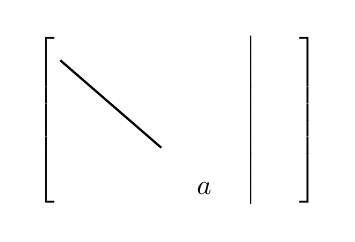
\begin{tikzpicture}[baseline=(current bounding box.center)]
                    % 放置矩阵
                    \node (mat) {
                        $\begin{bmatrix}
                             \; & \; & \; & \; & \; & \;\big|\; & \; \\
                             \; & \; & \; & \; & \; & \;\big|\; & \; \\
                             \; & \; & \; & \; & \; & \;\big|\; & \; \\
                             \; & \; & \; & \; & \; & \;\big|\; & \; \\
                             \; & \; & \; & \; & a  & \;\big|\; &
                        \end{bmatrix}$
                    };

                    % 画主对角线
                    % 从矩阵左上角到右下角(倒数第二列)
                    \draw[thick,black]
                    ([xshift=12pt,yshift=-12pt]mat.north west) --
                    ([xshift=-60pt,yshift=24pt]mat.south east);
                \end{tikzpicture}
            \]
            若$a = 0$则{\color{red}{有可能}}无解
            \begin{enumerate}
                \item $\forall a$均有解
                \[
                    \bar{A} =
                    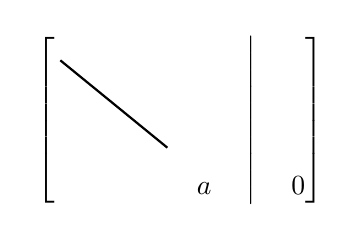
\begin{tikzpicture}[baseline=(current bounding box.center)]
                        % 放置矩阵
                        \node (mat) {
                            $\begin{bmatrix}
                                 \; & \; & \; & \; & \; & \;\big|\; & \; \\
                                 \; & \; & \; & \; & \; & \;\big|\; & \; \\
                                 \; & \; & \; & \; & \; & \;\big|\; & \; \\
                                 \; & \; & \; & \; & \; & \;\big|\; & \; \\
                                 \; & \; & \; & \; & a  & \;\big|\; & 0
                            \end{bmatrix}$
                        };

                        % 画主对角线
                        % 从矩阵左上角到右下角(倒数第二列)
                        \draw[thick,black]
                        ([xshift=12pt,yshift=-12pt]mat.north west) --
                        ([xshift=-60pt,yshift=24pt]mat.south east);
                    \end{tikzpicture}
                \] \\
                \item 若$b \neq 0$必无解
                \[
                    \bar{A} =
                    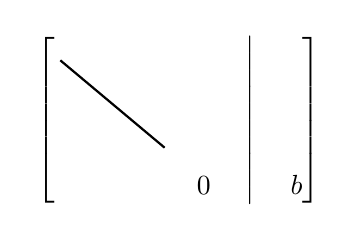
\begin{tikzpicture}[baseline=(current bounding box.center)]
                        % 放置矩阵
                        \node (mat) {
                            $\begin{bmatrix}
                                 \; & \; & \; & \; & \; & \;\big|\; & \; \\
                                 \; & \; & \; & \; & \; & \;\big|\; & \; \\
                                 \; & \; & \; & \; & \; & \;\big|\; & \; \\
                                 \; & \; & \; & \; & \; & \;\big|\; & \; \\
                                 \; & \; & \; & \; & 0  & \;\big|\; & b
                            \end{bmatrix}$
                        };

                        % 画主对角线
                        % 从矩阵左上角到右下角(倒数第二列)
                        \draw[thick,black]
                        ([xshift=12pt,yshift=-12pt]mat.north west) --
                        ([xshift=-60pt,yshift=24pt]mat.south east);
                    \end{tikzpicture}
                \]
            \end{enumerate}
            \item \emph{e.g.}
            \[
                \left[
                    \begin{array}{ccc|c}
                        1 & -1              & a                & 2   \\
                        & \underline{a-1} & a+2              & -3  \\
                        &                 & \underline{2a+6} & a-9
                    \end{array}
                    \right]
            \]
            从下向上依次检查与$0$的关系
            \begin{enumerate}
                \item 先看$2a + 6 = 0$
                \item 再看$a - 1 = 0$
            \end{enumerate}
            \begin{align*}
                & \text{唯一解} && \Leftrightarrow r(A) = r(\bar{A}) = n && \Leftrightarrow a \neq 1 \text{ 且 } a \neq -3 \\
                & \text{无穷解} && \Leftrightarrow r(A) = r(\bar{A}) < n && \Leftrightarrow a = 1 \\
                & \text{无解}   && \Leftrightarrow r(A) + 1 = r(\bar{A}) && \Leftrightarrow a = -3
            \end{align*}
        \end{enumerate}
        \item 证明$\alpha_1,\alpha_2,\dots,\alpha_t$是$Ax = 0$的基础解系,需要
        \begin{enumerate}
            \item 验证$\alpha_1,\alpha_2,\dots,\alpha_t$是$Ax = 0$的解
            \item 证明$\alpha_1,\alpha_2,\dots,\alpha_t$线性无关
            \item $t = n - r(A)$
        \end{enumerate}
        \item 非齐次线性方程组求解方法
        \begin{enumerate}
            \item 对增广矩阵作初等{\color{red}{行变换}}化为阶梯形矩阵
            \item 求导出组的几个基础解系
            \item 求方程组的一个特解(为简捷,可令自由变量全为0)
            \item 按解的结构写出通解
            \item 注: \textbf{当方程组中含有参数时,分析讨论要严谨不要丢情况}
        \end{enumerate}
        \item 公共解处理方法(例4.16)
        \begin{enumerate}
            \item (I)(II)联立求解
            \item 通过(I)与(II)各自的通解,寻找非零公共解
            \item 把(I)的通解带入(II)中,如果仍是解,寻找$k_1, k_2$所对应满足的关系式而求出公共解
        \end{enumerate}
        \item 证明两方程同解
        \begin{enumerate}
            \item 定义
            \item $r(A) = r(B)$且$Ax = 0$ 的解全是 $Bx = 0$的解
        \end{enumerate}
    \end{enumerate}

    \subsection{条件转换思路}
    \begin{enumerate}
        \item 抽象方程组(例4.9)
        \begin{enumerate}
            \item 解的结构
            \item 解的性质
            \item 秩
        \end{enumerate}
    \end{enumerate}

    \subsection{理解}

    \begin{enumerate}
    \end{enumerate}


\end{document}
